%!TEX program = <xelatex>
\documentclass[xetex]{beamer}
% \documentclass[draft, xetex]{beamer}

		% Iclude packages and commands used text-wide.	
%%%%%%%%%%%%%%%%%%%%%%%%%%%%%%%%%%%%%%%%%%%%%%%%%%%%%%%%%%%%%%%%%%%%%%%%%%%%%%%%%%%%%%%%%%%%%%%%%%%%%%%%%%%

\usepackage{mystyle}

		% Presentation settings.
%%%%%%%%%%%%%%%%%%%%%%%%%%%%%%%%%%%%%%%%%%%%%%%%%%%%%%%%%%%%%%%%%%%%%%%%%%%%%%%%%%%%%%%%%%%%%%%%%%%%%%%%%%%


		% Title
	\title[Parrellel Tempering]{Parrellel Tempering }
	\subtitle{Master Thesis Defense}

	\date{14 January 2014} 
	\author[Łącki]{Mateusz Łącki}
	\institute[UW]{Uniwersytet Warszawski}
	\titlegraphic{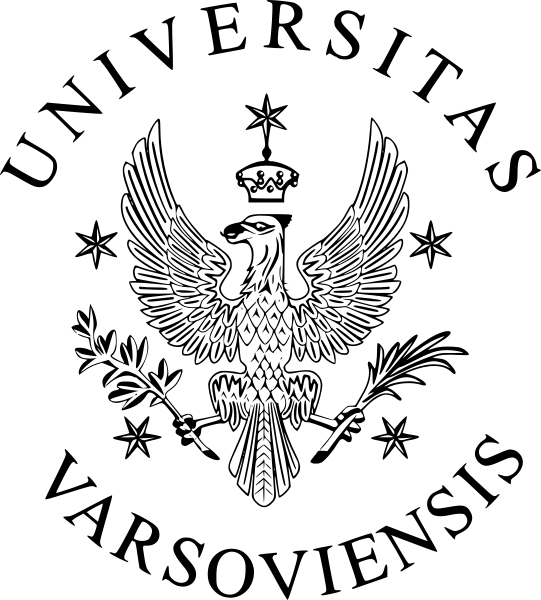
\includegraphics[scale=.10 , keepaspectratio]{./picts/eagle3.png}}
	
		% The document
%%%%%%%%%%%%%%%%%%%%%%%%%%%%%%%%%%%%%%%%%%%%%%%%%%%%%%%%%%%%%%%%%%%%%%%%%%%%%%%%%%%%%%%%%%%%%%%%%%%%%%%%%%%	

\begin{document}

	\fontspec[Numbers={OldStyle}]{Linux Libertine O}

	%%%%%%%%%%%%%%%%%%%%%%%%%%%%%%%%%%%%%%%%%%%%%%%%%%%%%%%%%%%%%%

	\begin{frame}
		\titlepage
	\end{frame}

	%%%%%%%%%%%%%%%%%%%%%%%%%%%%%%%%%%%%%%%%%%%%%%%%%%%%%%%%%%%%%%

	\begin{frame}
		\frametitle{Today's Agenda}
		\tableofcontents
	\end{frame}

	%%%%%%%%%%%%%%%%%%%%%%%%%%%%%%%%%%%%%%%%%%%%%%%%%%%%%%%%%%%%%%
\section{Motivation}
	%%%%%%%%%%%%%%%%%%%%%%%%%%%%%%%%%%%%%%%%%%%%%%%%%%%%%%%%%%%%%%


	\begin{frame}[t]\frametitle{The Metropolis-Hastings Algorithm}
	    
		\begin{itemize}
			\item[Goal] 	Generate a representatative sample
			\item[Mean]		Searching state-space for probability clusters in 2 steps
			\begin{enumerate}
				\item 	Choose $x_0$ in any way

				\item  	Given previous step $X^{[n-1]} = x^{[n-1]}$, draw proposal
					$$ Y \sim \mathcal{Q}(x^{[n-1]}, \circ) $$

				\item 	Draw
					$$ U \sim \mathcal{U}(0,1) $$	

				\item 	Accept the proposal ($X_{n} := Y$) if 
					$$ U \leq \alpha(x^{[n-1]},Y) $$
				\item[where] $\alpha (x^{[n-1]},y) = 1 \wedge \frac{\pi(y)}{\pi(x^{[n-1]})}$ 
			\end{enumerate}

		\end{itemize}
	
	\end{frame}

	%%%%%%%%%%%%%%%%%%%%%%%%%%%%%%%%%%%%%%%%%%%%%%%%%%%%%%%%%%%%%%

	\begin{frame}[t]\frametitle{Problems with Metropolis-Hastings}
	    	
		\begin{itemize}
			\item Choice of $\alpha$ : self-adjointess of corresponding kernel:
				$$ \mathcal{M}(x, A) = \underbrace{\int_A \alpha(x,y) \mathcal{Q}(x, \mathrm{d}\,y)}_{\prob \Big( X^{[n+1]}\not=x \,\,\text{and}\,\, X^{[n+1]} \in A \Big) } + \,
				\mathbb{I}_A(x) \underbrace{\int \Big(1- \alpha(x,y)\Big) \mathcal{Q}(x, \mathrm{d}\,y)}_{\prob \Big( X^{[n+1]} = x\Big)}$$
			\begin{itemize}
				\item Kernel preserves the distribution $\pi(x)\mathrm{d}\,x$
			\end{itemize}

			\item Problem: $\frac{\pi(y)}{\pi(x^{[n-1]})}$
			\begin{itemize}
				\item 	 promotes acceptances of points with not so much smaller probability
			\end{itemize}

			\item[If] 	$\mathcal{Q}(x,\circ)$ centered to much around $x$, 
			\item[then] Difficult to leave $x$'s surroundings.
		\end{itemize}
	
	\end{frame}


	%%%%%%%%%%%%%%%%%%%%%%%%%%%%%%%%%%%%%%%%%%%%%%%%%%%%%%%%%%%%%%

	\begin{frame}[t]\frametitle{Liang-Wang Example}

		\begin{itemize}
			\item[] 	Metropolis-Hastings algorithm's flaw: \textsc{Localness}
			\item[] 	$$ f(x) = 
				\sum_{i=1}^{20} \frac{\omega_i}{ \sigma_i \sqrt{2 \pi} } \exp \Big( -\frac{(x - \mu_i)'(x - \mu_i)}{2 \sigma_i^2} \Big) $$
			\item[]
			\item[] 	where $\sigma_1 = \dots = \sigma_{20} = 0.1$, $\omega_1 = \dots = \omega_{20} = 0.05 $
			\item[] 	and the means $\mu_i$ are given by
			\item[] 
			\begin{table}[ht]
				\centering
				\begin{tabular}{rrrrrrrrrr}
				  \hline
					1 & 2 & 3 & 4 & 5 & 6 & 7 & 8 & 9 & 10 \\ 
				  \hline
					2.18 & 8.67 & 4.24 & 8.41 & 3.93 & 3.25 & 1.70 & 4.59 & 6.91 & 6.87 \\ 
				  	5.76 & 9.59 & 8.48 & 1.68 & 8.82 & 3.47 & 0.50 & 5.60 & 5.81 & 5.40 \\ 
				   \hline
				\end{tabular}
			\end{table}
			\item[]
			\begin{table}[ht]
				\centering
				\begin{tabular}{rrrrrrrrrr}
				  \hline
					11 & 12 & 13 & 14 & 15 & 16 & 17 & 18 & 19 & 20 \\ 
				  \hline
					5.41 & 2.70 & 4.98 & 1.14 & 8.33 & 4.93 & 1.83 & 2.26 & 5.54 & 1.69 \\ 
					2.65 & 7.88 & 3.70 & 2.39 & 9.50 & 1.50 & 0.09 & 0.31 & 6.86 & 8.11 \\ 
				   \hline
				\end{tabular}
			\end{table}
		\end{itemize} 			
	
	\end{frame}

	%%%%%%%%%%%%%%%%%%%%%%%%%%%%%%%%%%%%%%%%%%%%%%%%%%%%%%%%%%%%%%

	\begin{frame}[t]\frametitle{Multimodial Disaster}

		\begin{center}
			\begin{figure}
				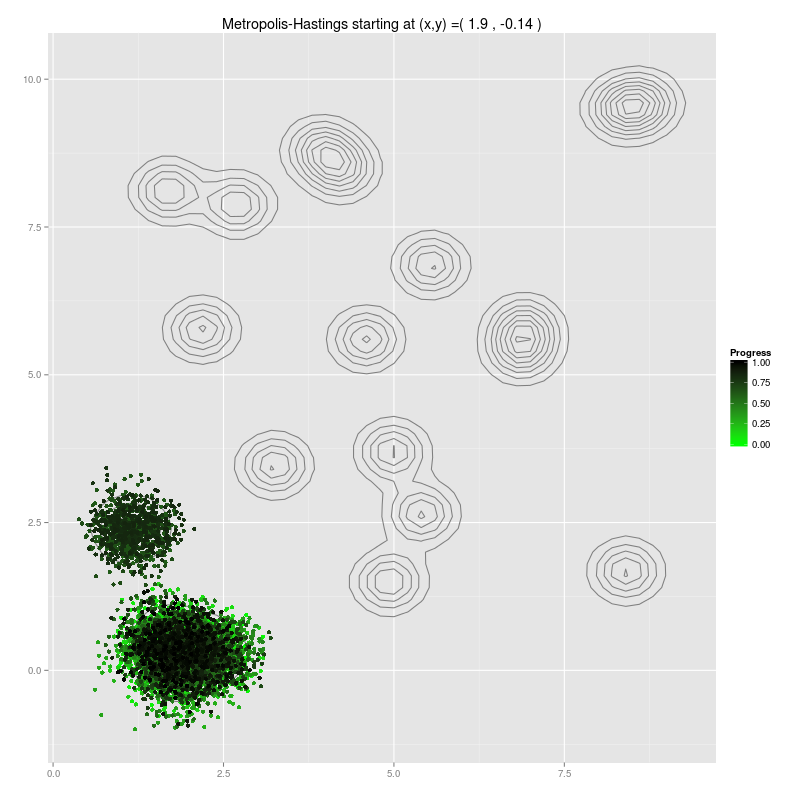
\includegraphics[height=.8\textheight, keepaspectratio]{./picts/MH_simululation_10000_steps.png}
			\end{figure}	
		\end{center}
 	
	\end{frame}

	%%%%%%%%%%%%%%%%%%%%%%%%%%%%%%%%%%%%%%%%%%%%%%%%%%%%%%%%%%%%%%
\section{The PT Algorithm}
	%%%%%%%%%%%%%%%%%%%%%%%%%%%%%%%%%%%%%%%%%%%%%%%%%%%%%%%%%%%%%%

	\begin{frame}[t]\frametitle{Solution: Parallel Tempering}    
		\begin{columns}
			\begin{column}[t]{.5\textwidth}
			    \begin{itemize}
			    	\item Enlarge the state-space!
			    	\begin{itemize}
			    		\item[Chain] 	$X^{[n]} 	= \Big( X^{[n]}_1, \dots, X^{[n]}_L \Big)$ 
			    		\item[Aim] 		$\pi_\beta 	\propto \pi^{\beta_1} \times \dots \times \pi^{\beta_L}$
			    		\begin{itemize}
			    			\item[where] $\underbrace{\beta = (\beta_1, \dots, \beta_L)}_\text{inverse temperatures}$ 
			    			\item[and] 	$\beta_1 \equiv 1$	 
			    		\end{itemize}
			    	\end{itemize}
			    	\item  	Move independently with each chain
			    	\item  	$\alpha_{\beta_l} = \Big(\frac{\pi(y)}{\pi(x)}\Big)^{\beta_l} > \frac{\pi(y)}{\pi(x)} = \alpha_{\beta_1} $
			    	\item[then]  	Exchange accepted proposals \dots
			    \end{itemize}
			\end{column}
			\begin{column}[t]{.5\textwidth}	
				\begin{center}
					\begin{figure}
						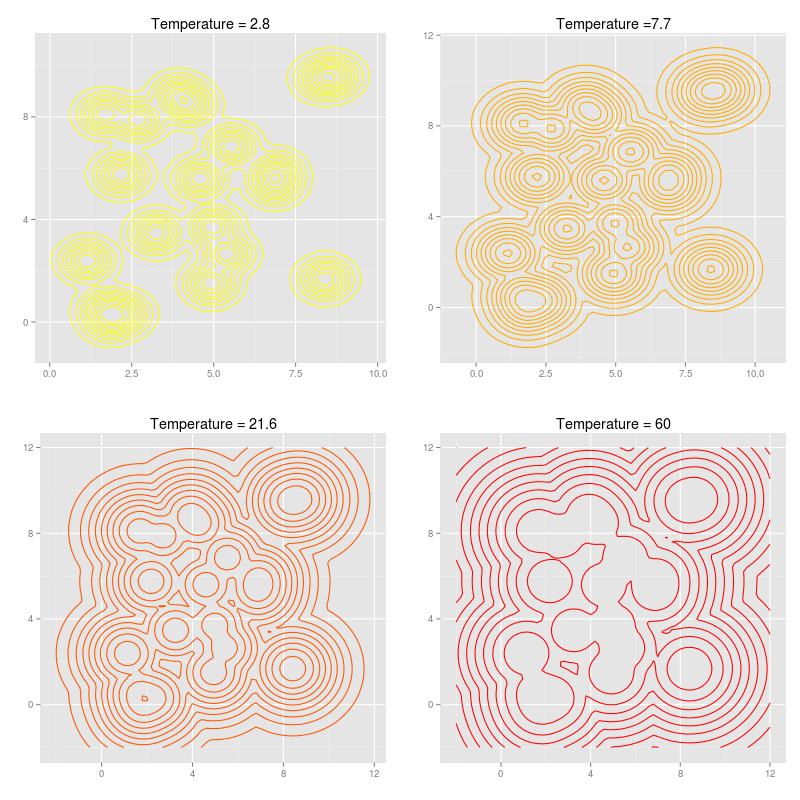
\includegraphics[width=\textwidth, keepaspectratio]{./picts/Liang_Contour_plots.png}
					\end{figure}	
				\end{center}
			\end{column}
		\end{columns}	
	\end{frame}

	%%%%%%%%%%%%%%%%%%%%%%%%%%%%%%%%%%%%%%%%%%%%%%%%%%%%%%%%%%%%%%

	\begin{frame}[t]\frametitle{Swaping proposals}
	    
		\begin{itemize}
			\item 	Last States:   	$x \equiv x^{[n-1]} 	= \Big( x^{[n-1]}_1, \dots, x^{[n-1]}_L \Big)$
			\item  	Proposal Kernel:   	$\mathcal{T}(x, A) \equiv \underset{i < j}{\sum} p_{ij}(x) \mathbb{I}_A (S_{ij} x)$
			\begin{itemize}
				\item[where] 	$S_{ij} x = (x_1, \dots, x_{i-1}, x_j, x_{i+1}, \dots, x_{j-1}, x_i, x_{j+1}, \dots, x_L)$	 
			\end{itemize}		
			
			\item To assure related kernel self-adjointness
			\begin{equation*}
				\alpha_\text{swap}(x,\underbrace{S_{ij} x}_\text{proposal}) = \Biggl[  \Big(\frac{\pi(x_j)}{\pi(x_i)} \Big)^{\beta_i - \beta_j}  \frac{ p_{ij}(S_{ij} x )}{ p_{ij}( x ) }\Biggl] \wedge 1
			\end{equation*}

			\item[So] different distributions on swaps = \textcolor{red}{\textsc{Strategies}}
			\item[Also] possibly state-dependent: $p_{ij} = p_{ij}(x)$
		\end{itemize}
	
	\end{frame}

	%%%%%%%%%%%%%%%%%%%%%%%%%%%%%%%%%%%%%%%%%%%%%%%%%%%%%%%%%%%%%%
\section{New Strategies}
	%%%%%%%%%%%%%%%%%%%%%%%%%%%%%%%%%%%%%%%%%%%%%%%%%%%%%%%%%%%%%%

	\begin{frame}[t]\frametitle{Our choices for \textcolor{red}{Strategies}}
	    
	   	\begin{columns} 
	    	\begin{column}[t]{.5\textwidth}	
				\begin{table}[htbp]
					\begin{tabular}{cc}
					\textcolor{red}{\textsc{Strategy}} & Proportional to \\ 
					&\\
					I &  $\frac{\pi (x_j)}{\pi( x_i )} \wedge \frac{\pi (x_i)}{\pi( x_j )}$ \\ 
					&\\
					II & $\frac{\pi (x_j)}{\pi( x_i )} \wedge 1$ \\ 
					&\\
					III & $\Big( \frac{\pi (x_j)}{\pi( x_i )} \wedge 
								\frac{\pi (	x_i)}{\pi( x_j )} \Big)^{|\beta_i - \beta_j|}$
					\end{tabular}
				\end{table}
			\end{column}
			\begin{column}[t]{.5\textwidth}			
				\begin{table}[htbp]
					\begin{tabular}{cc}
					\textcolor{red}{\textsc{Strategy}} & Proportional to \\ 
					IV & $\Big( \frac{\pi (x_j)}{\pi( x_i )} \wedge \frac{\pi (x_i)}{\pi( x_j )} \Big)^\frac{|\beta_i - \beta_j|}{1 + \rho(x_i, x_j)}$ \\ 
					&\\
					V & $\frac{2}{L (L - 1)}$ \\ 
					&\\
					VI & $\frac{1}{L - 1} \ind{\{|i-j|=1\}}$ \\ 
					\end{tabular}
				\end{table}
			\end{column}
		\end{columns}	
	\end{frame}


	%%%%%%%%%%%%%%%%%%%%%%%%%%%%%%%%%%%%%%%%%%%%%%%%%%%%%%%%%%%%%%
\section{Results}
	%%%%%%%%%%%%%%%%%%%%%%%%%%%%%%%%%%%%%%%%%%%%%%%%%%%%%%%%%%%%%%
	



	%%%%%%%%%%%%%%%%%%%%%%%%%%%%%%%%%%%%%%%%%%%%%%%%%%%%%%%%%%%%%%	
\section{The Template}
	%%%%%%%%%%%%%%%%%%%%%%%%%%%%%%%%%%%%%%%%%%%%%%%%%%%%%%%%%%%%%%




	%%%%%%%%%%%%%%%%%%%%%%%%%%%%%%%%%%%%%%%%%%%%%%%%%%%%%%%%%%%%%%
\section{Other Minor Implementations}
	%%%%%%%%%%%%%%%%%%%%%%%%%%%%%%%%%%%%%%%%%%%%%%%%%%%%%%%%%%%%%%




	%%%%%%%%%%%%%%%%%%%%%%%%%%%%%%%%%%%%%%%%%%%%%%%%%%%%%%%%%%%%%%
\section{Future Research}
	%%%%%%%%%%%%%%%%%%%%%%%%%%%%%%%%%%%%%%%%%%%%%%%%%%%%%%%%%%%%%%









	%%%%%%%%%%%%%%%%%%%%%%%%%%%%%%%%%%%%%%%%%%%%%%%%%%%%%%%%%%%%%%
\end{document}
  
  
%%%%%%%%%%%%%%%%%%%%%%%%%%%%%%%%%%%%%%%%%%%%%%%%%%%%%%%%%%%%%%%%%%%%%%%%%%%

